\documentclass[a5paper,fontsize=10pt]{memoir}
\usepackage[
  top=2cm,bottom=2cm,
  inner=1.75cm,
  outer=1.25cm,
  textwidth=13cm
]{geometry}
\strictpagecheck

\usepackage[utf8]{inputenc}
\usepackage[german]{babel}

\usepackage{palatino}
\usepackage[T1]{fontenc}

\usepackage{graphicx}
\usepackage{fancyhdr}
\usepackage{hyphenat}
\usepackage{svg}
\usepackage{xr-hyper}
\usepackage{hyperref}
\usepackage{tikz}
\usepackage{xfrac}
\usepackage{marvosym}
\usepackage{lmodern,xspace}
\usepackage{ziffer}
\usepackage{numprint}
\usepackage{xfp}
\usepackage[nomessages]{fp}

\externaldocument{transcription}
\interfootnotelinepenalty=10000

\renewcommand{\headrulewidth}{0pt}
\pagestyle{fancyplain} % Makes all pages in the document conform to the custom headers and footers
\fancyhead[L]{}% Empty left header
\fancyhead[C]{\thepage} % Page numbering for center header
\fancyhead[R]{}% Empty right header
\fancyfoot[L]{}% Empty left footer
\fancyfoot[C]{}% Empty center footer
\fancyfoot[R]{}% Empty left footer


\makeatletter
\newcommand*{\addFileDependency}[1]{% argument=file name and extension
  \typeout{(#1)}
  \@addtofilelist{#1}
  \IfFileExists{#1}{}{\typeout{No file #1.}}
}
\makeatother

\newcommand*{\myexternaldocument}[1]{%
    \externaldocument{#1}%
    \addFileDependency{#1.tex}%
    \addFileDependency{#1.aux}%
}

\myexternaldocument{transcription}

%\newcommand\ouncesofpound{16}
%\newcommand\quentinsofounce{7}
%\newcommand\gransofquentins{54}
%\newcommand\gramsofpound{378}

\newcommand\ouncesofpound{12}
\newcommand\quentinsofounce{8}
\newcommand\gransofquentins{63}
\newcommand\gramsofpound{372}

\newcommand\literofpound{\fpeval{\gramsofpound / 1000}}
\newcommand\gramofounce{\fpeval{\gramsofpound / \ouncesofpound}}
\newcommand\gramofquentin{\fpeval{\gramsofpound / \ouncesofpound / \quentinsofounce}}
\newcommand\gramofgran{\fpeval{\gramsofpound / \ouncesofpound / \quentinsofounce / \gransofquentins}}

\newcommand\cubiccmofcubicinch{19.8364}

\begin{document}

{\centering
{\Large Anhang}
\vspace{2em}

\begin{minipage}{4cm}
  \hrulefill\\
\end{minipage}

}

\section{Zu den Maßeinheiten}

Auf Seite \pageref{units_value_page} gibt
v. Stipriaan Luïsçius
Hinweise auf die tatsächlich anzuwendende Umrechnung.
Er gibt an,
dass 5 \sfrac{1}{3} Quentchen insgesamt 330 Gran,
sowie 3 Quentchen 40 Gran 220 Gran seien.
Rechnerisch bedeutet das%
\footnote{330 Gran / 62 = 5,32 Quentchen,
resp. 3 * 60 Grane + 40 Gran = 220 Grane}%
, dass 1 Quentchen insgesamt 60 oder 62 sind,
wofür ich z.B. auf wikipedia.org keinerlei Hinweise gefunden habe.

Folgende Bücher habe ich zu diesem Thema gefunden
und zum Vergleich herangezogen:
\begin{itemize}
\item \emph{Philologisch-kritischer u. historischer Commentar
über die drey ersten Evangelien, Zweyter Theil}
von Heinrich Eberhard Gottlob Paulus%
\footnote{\href{https://books.google.de/books?id=-WPPudKsXE8C}
{books.google.de/books?id=-WPPudKsXE8C}}
\item \emph{Metrologische Tafeln über die alten Maaße,
Gewichte und Münzen Roms und Griechenlands}
nach Romé de l'Isle,
übersetzte von G. Große%
\footnote{\href{https://books.google.de/books?id=DGs6AAAAcAAJ}
{books.google.de/books?id=DGs6AAAAcAAJ}}
\item \emph{Johann Potters griechische Archäologie,
oder, Alterthümer Griechenlandes.
Aus dem Engländischen übersetzt
und mit Anmerkungen und Zusätzen vermehrt, Dritter Theil}
von John Potter%
\footnote{\href{https://books.google.de/books?id=DQdAAQAAMAAJ}{books.google.de/books?id=DQdAAQAAMAAJ}}
\end{itemize}
In diesen konnte ich Referenzen zu annähernden Wertentsprechungen finden.
Von \emph{Gottlob Paulus} heißt es auf den Seiten 679 u. 680:\\

\emph{«Franz. Perez Bayer de numis hebraeo - samaritanis (1781.)
welcher hier vorn. zu vergleichen wäre,
fand nach dem Gewicht des vorhandenen Schekel
mit hebr. samaritanischer Inschrift,
daß ein ganzer von Silber
252 = viermal 63 grana (span. Apothekergewicht) wiegt,
folgl. eine attische Drachme gerade 63 Gran gewogen habe.»}\\

\emph{De l'Isle} schreibt auf Seite 25 in Fußnote p):\\

\emph{«Man sehe die obengedachten verschiedenen Systeme.
Jacob Lapelle aber macht hier eine Ausnahme.
Dieser gibt sogar dem Römischen Pfunde den Namen eines Attischen,
und legt bei der Werthbestimmung einer Drachme
einen Denar von 63 Gran zum Grunde.»}\\

%Denmach ist anzunehmen das A. v. Stipriaan Luïsçius ein im ersten Zitat angedeutetes Gewichte-Set besessen und/oder diese römische resp. attische Rechengrundlage verwendet haben muss.
Ausgehend von 63 Gran pro Quentchen
und der in dem Zusammenhang erwähnten 252 Gran pro Silberschekel
kommt man auf einen Wert von 6048 Gran pro römisches Pfund,
was sich folgendermaßen herleiten lässt:\\

\noindent
\begin{minipage}{\linewidth}
\footnotesize
\FPeval\scruplesofquentins{21} %round((63/3):0}
\begin{tabbing}
Zeroooo  \= Oneeeeeeeeeeeee \= Twoooooooooooo    \= Threeeeeeeeeeeeeeee \= Fourrrrrrrrrrrrrrrrrr \= Five      \kill
         \>  \'             \>  \'               \> 1\'Drachme          \>   3\'Skrupel (x\scruplesofquentins)    \>  63\'Gran \\
         \>  \'             \> 1\'Silberschekel  \> 4\'Drachmen (x\gransofquentins)   \>  12\'Skrupel (x\scruplesofquentins)    \> 252\'Gran \\
         \> 1\'Unze         \> 2\'Silbers.(x252) \> 8\'Drachmen (x\gransofquentins)   \>  24\'Skrupel (x\scruplesofquentins)    \> 504\'Gran \\
1 \Pfund \>12\'Unzen (x504) \>24\'Silbers.(x252) \>96\'Drachmen (x\gransofquentins)   \> 288\'Skrupel (x\scruplesofquentins)    \>6048\'Gran \\
\end{tabbing}
\end{minipage}

Auf den Wert 6048 kommt auch  Romé de l'Ilse
für das römische Pfund%
\footnote{Siehe Seite VII der Vorrede des Übersetzers.},
jedoch auf eigenem Wege der Gewichtsbestimmung,
ohne mit 252 Gran als Basiswert
für ein Silberschekel (vier Drachmen) zu arbeiten.
Hofrath Kästner korrigiert im Anhang mathematisch
den Wert eines römischen Pfundes auf 6024,1 Gran.
Allerdins schreibt er auch:\\

\emph{«Den bei diesen Unsicherheiten des römischen Maaßes
und Gewichtes in kleinen Theilen,
beruhigt mich der Ausspruch eines zuverlässigen Richters:
daß wir mit allen Bemühungen der Scholiasten, Grammatiker und Kritiker,
Homers Gesänge nie so zu lesen bekommen,
wie die Griechen sie gehört haben.»}\\

Weiterhin heißt es auf Seite VIII der Vorrede des Übersetzers:\\

\emph{«Folglich ist des Verfassers durch Abwiegung
alter Goldmünzen gefundenes römisches Pfund genau dasselbe,
das man durch die obige Berechnung erhält
und muß daher das richtige und Wahre sein.»}\\

Im dritterwähnten Buch von Johann Potters
heißt es auf Seite 155:\\

\emph{«Eben diese Summe%
\footnote{744 Pence = 5952 Gran bzw. 1 Pence = 8 Gran,
gemäß englischem Troygewicht nach Greaves}
kommt dann schon heraus,
wenn man jeder attischen Drachme nur die 62 Gran giebt,
die nach Greaves Anzeige der römische Denar gehabt hat,
und wenn man die \texttt{libram argenti} nur auf 96 Drachmen
oder Denarien rechnet.
Denn 96 mit 62 multiplicirt macht 5952.
Und in der That sind nach der \texttt{libra medica},
die aus 12 Unzen bestand, 96 Drachnen oder Denarien,
deren jede den achten Theil einer Unze enthielt,
aufs Pfund gerechnet worden;
so wie nach der \texttt{libra ponderali} nur 84 Drachmen
oder Denarien dazu gezählt wurden,
in so fern jede Drachme den siebenten Theil einer Unze ausmachte.»}\\

62 Gran pro Quentchen ist der
-- bzgl. der von A. v. Stipriaan Luïsçius angestellten Untersuchungen%
\footnote{Für 63 Gran pro Quentchen
hätte er 5\sfrac{1}{4} anstatt 5\sfrac{1}{3} Quentchen
für 330 Gran angeben müssen,
resp. 3 Qu. 40 Gr. hätten 226 oder 229 Gran ergeben müssen,
wären 62 resp. 63 Gran die Basis für ein Quentchen.}%
-- am nahe liegendste Wert,
zu dem ich eine Referenz finden konnte,
Allerdings erscheint mir der Wert von 63 Gran pro Quentchen
-- wie im obigen Zitat erwähnt
-- der wahre zu sein,
und kleinere Abweichungen in den Mess- bzw. Kontrollgewichten
%kleinere Messfehler bzw. Übertragungsfehler Seitens Luïsçius
sind auch nicht ganz auszuschließen. Daher entschied ich mich dazu,
für alle weiteren Berechnungen 
von eben diesen 63 Gran pro Quentchen auszugehen. 
Das heißt also für die Übersicht:\\

\noindent
\begin{minipage}{\linewidth}
\begin{tabbing}
Zerooooooo \= Oneeeeeeeeeeeeeeeeee \= Twoooooooooooooooooooo \= Three      \kill
           \>  \'                  \> 1\'Drachme             \>  \gransofquentins\'Gran \\
           \> 1\'Unze              \> \quentinsofounce\'Drachmen (x\gransofquentins)      \> \fpeval{\quentinsofounce * \gransofquentins}\'Gran \\
1 \Pfund   \>\ouncesofpound\'Unzen (x\fpeval{\quentinsofounce * \gransofquentins})      \>\fpeval{\ouncesofpound * \quentinsofounce}\'Drachmen (x\gransofquentins)      \>\fpeval{\ouncesofpound * \quentinsofounce * \gransofquentins}\'Gran \\
\end{tabbing}
\end{minipage}

Im damaligen Königreich Niederlande
betrug 1 Pfund Medizinalgewicht 375 Gramm
(eingeführt 1. Januar 1820).%
\footnote{\href{https://web.archive.org/web/20160817163942/https://de.wikipedia.org/wiki/Apothekergewicht}
{de.wikipedia.org/wiki/Apothekergewicht}}

Eine Rechnung mit den historisch korrekten 372 Gramm 
ergibt bei den nachfolgend errechneten Werten 
allerdings kaum eine Änderung, 
weshalb ich mich für diesen Wert 
als Basis für die Umrechnungen entschieden habe.

Aus dem Zitat des letzterwähnten Buches kann man erkennen,
dass das Medizinalpfund (\texttt{libra medica}) 12 Unzen hatte,
das Handelspfund (\texttt{libra ponderali}) hingegen 16 Unzen bemaß.

Für die nachfolgenden Umrechnungen seiner Untersuchungsergebnisse
verwende ich somit folgende Werte in der metrischen Einheit Gramm:\\

\noindent
\begin{minipage}{\linewidth}
\FPeval\x{round(\gramofquentin:3)}
\FPeval\y{round(\gramofgran:3)}
\begin{tabbing}
Zr \= Oneeeeeeeeeeeeeeeeeeeeeee \= Twooo                 \kill
   \>1\'Pfund (\Pfund)        \>\numprint{\gramsofpound}\'Gramm oder \sfrac{3}{8} Liter Wasser\\
   \>1\'Unze                  \>\numprint{\gramofounce}\'Gramm\\
   \>1\'Quentchen             \>\numprint{\x}\'Gramm\\
   \>1\'Gran                  \>\numprint{\y}\'Gramm\\
\end{tabbing}
\end{minipage}

\FPeval\x{round(4*\literofpound:1)}
\FPeval\y{round(330*\gramofgran:2)}
Wenn also z.B. von 4 \Pfund\kern+0.14em Wasser die Rede ist,
ergeben sich daraus umgerechnet \numprint{\x} Liter;
bei bspw. 330 Gran ergeben sich umgerechnet \numprint{\y} Gramm.

% 1 Kubikzoll (Pariser) = \sfrac{10}{9} Kubikzoll (Rheinl.) = 19,8364 cm³ = ca. 1/50000 m³%
Da nicht eindeutig aus dem Dokument hervorgeht,
welches Kubikzoll verwendet wurde,
gehe ich vorerst vom weiter verbreiteten pariser Kubikzoll aus.
Ein solches sind \sfrac{10}{9} rheinländischen Kubikzollen,
was umgerechnet \mbox{\numprint{\cubiccmofcubicinch} cm³} oder ca. 1/50000 m³ entspricht.%
\footnote{\href{https://web.archive.org/web/20210919211741/https://de.wikipedia.org/wiki/Pariser_Kubikzoll}
{de.wikipedia.org/wiki/Pariser\textunderscore Kubikzoll}}
%-- zumal es für seine eigenen Untersuchungen nicht von Belang ist.
%\vfill

\section{Analyse}

\FPeval\x{round(2*\gramofquentin:0)}%
Als einfachste Weise,
Natriumhydrogencarbonat dem Körper zuzuführen,
wird angeführt,\xspace
\mbox{ca. \numprint{\x} Gramm} Natron in einen halben Liter Wasser zu geben
und von der Lösung jeweils einen Löffel seinem Trinkwasser hinzuzufügen 
-- zum Beispiel ein Teelöffel auf ein Glas gutes Wasser.

\FPeval\x{round(4*\literofpound:1)}%
Es wird dann hervorgehoben,
dass das Fachinger Wasser an sich schon
einen vergleichsweise hohen Anteil an Natron beinhaltet,
wobei Geschmack und Konsistenz einem neutralen, stillen Wasser gleichen.
Die inhaltlichen Bestandteile des damaligen Fachinger Wassers
wurden wie folgt von Wuth%
\footnote{\emph{De Aqua Soteria Fachingensi. 
Dissertatio Inauguralis Physico-Medica} von 1779\\
(\href{https://books.google.de/books?id=vq5TAAAAcAAJ}
{books.google.de/books?id=vq5TAAAAcAAJ})}
bemessen. Auf \numprint{\x} Liter Wasser kommen demnach:

\FPeval\salta{round(5*\gramofgran*1000:0)}%
\FPeval\saltb{round(11*\gramofgran*1000:0)}%
\FPeval\saltc{round(1*\gramofgran*1000:0)}%
\FPeval\saltd{round(3*\gramofgran*1000:0)}%
\FPeval\salte{round(3*\gramofgran*1000:0)}%
\FPeval\saltx{round(90*\gramofgran:1)}%
\begin{tabbing}
Zeroo \= One \= Two \= Three \kill
\>\FPeval\x{round(110*\cubiccmofcubicinch:0)}\numprint{\x}\' cm$^3$ \> Kohlenstoffdioxid bzw. Kohlensäure \\
\>\numprint{\salta}\' mg \> gewöhnliches Kochsalz\\
\>\numprint{\saltb}\' mg \> Calciumoxid bzw. Kalkerde\\
\>\numprint{\saltc}\' mg \> Magnesiumsulfat bzw. Bittersalz\\
\>\numprint{\saltd}\' mg \> Selenit bzw. Lithium\\
\>\numprint{\salte}\' mg \> Eisen[sulfit?]\\
\>\numprint{\saltx}\' g \> Kaliumhydrogencarbonat bzw. Weinsteinöl
\end{tabbing}

Säuren und Basen gleichen sich geschmacklich aus,
chemisch bleiben ihre Bestandteile vorhanden.
Bei hohem Kohlendioxid-Gehalt
kann eine entsprechend höhere Menge an Pottasche
(oder Natron)
hinzugefügt werden, wodurch
ein höherer Hydrogencarbonat-Anteil entsteht.
In dem beschriebenen Fall konnten
\FPeval\x{round(90*\gramofgran:1)}%
\FPeval\y{round(180*\gramofgran:1)}%
noch \mbox{\numprint{\x} g} Pottasche bzw. \mbox{\numprint{\y} g} Natron
dem gewöhlichen Fachinger Wasser hinugefügt werden
ohne dass der Geschmack unangenehm würde
oder sich andere Schwebstoffe später
nicht wieder mit der Kohlensäure verbunden hätten.
\FPeval\a{round(16*\gramofounce:0)}%
\FPeval\x{round(22.5*\gramofgran*1000:0)}%
%\FPeval\y{round(67*\gramofgran*1000:0)}%
\FPeval\y{round(((\x*2)+\salta+\saltb+\saltc+\saltd+\salte)/1000:1)}%
So hatte man schließlich auf \mbox{\numprint{\a} ml} Wasser
\mbox{\numprint{\x} mg} natürliches
und \mbox{\numprint{\x} mg} künstlich hinzugefügtes Kaliumcarbonat,
bzw. insgesamt -- incl. Kochsalz, Kalkerde, Bittersalz, Lithium und Eisensalz 
-- \mbox{ca. \numprint{\y} g} Mineralsalze.

Für größt mögliche Flexibilität in der Anwendung wird hier vorgeschlagen,
selber das Kaluimcarbonat mit Kohlensäure so zu sättigen,
dass man ein Mineralsalz erhält,
welches nach Bedarf dem Wasser hinzugefügt werden kann.\\

Die Herstellung dieses Salzes erfolgte wohl folgendermaßen:

\begin{center}
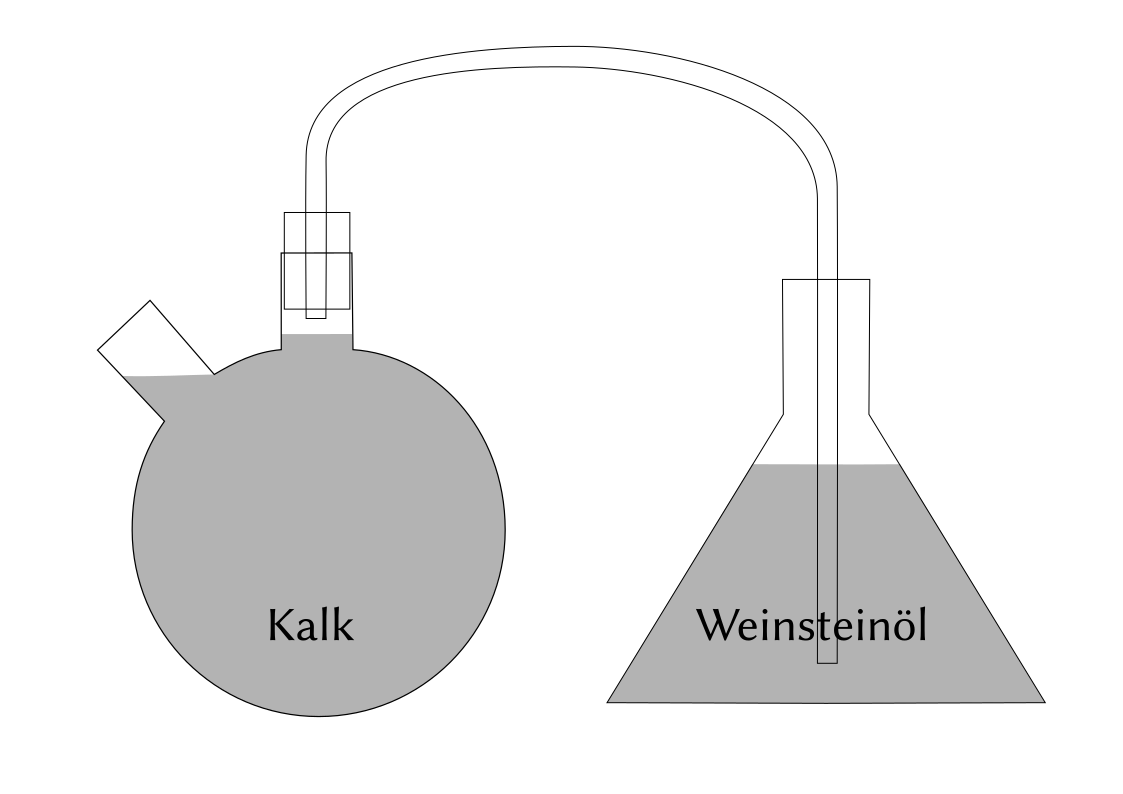
\includegraphics[width=6cm]{../figures/setting.png}
%\includesvg[width = 6cm]{figures/setting}
\end{center}

Bei diesem Aufbau blies er vermutlich mit dem Mund in die zweite Öffnung
des linken Behälters.
Die Kreide hatte hierbei die Funktion,
das Wasser aus dem Atem zu binden,
sodass oben durch das Glasröhrchen
nur noch das ausgeatmete CO$_2$ stömen konnte.
Dieses CO$_2$ strömte dann in das Weinsteinöl%
\footnote{Weinsteinöl = mit Wasserstoff gesättigtes Kaliumcarbonat
(HK$_2$CO$_3$?).\\
Zitat Wikipedia (\href{https://web.archive.org/web/20210724235820/https://de.wikipedia.org/wiki/Weinstein}
{de.wikipedia.org/wiki/Weinstein}):
\emph{Als dickflüssige Weinsteinlösung
bezeichnet man den Rückstand [aus der Wein-Herstellung],
bestehend aus Kaliumcarbonat und Kohle,
der infolge der Hygroskopie des Kaliumcarbonats
Wasser aus der Luft anzieht, an der Luft zerfließt
und daher zerflossenes Weinsteinöl genannt wurde.}}
des zweiten Behältnisses,
in welchem sich dann in der Reaktion
[Kaliumcarbonat-?]Kristalle bildeten,%
\footnote{Annahme:\\
2 KHCO$_3$ + CO$_2$ = K$_2$C$_2$O$_5$ + H$_2$O (Wasser)\\
Wobei sich das K$_2$C$_2$O$_5$ Salz an der Oberfläche der Lösung 
und dem Glasrand gebildet hat,
während sich das Wasser vermutlich am Boden des Behältnisses sammelte.}
die man dann von der Oberfläche des Weinsteinöls,
sowie der Innenwand des Glasbehälters entnehmen konnte 
und auf Löschpapier getrocknet hat.

\FPeval\a{round(16*\gramofounce:0)}%
\FPeval\x{round(80*\gramofgran:1)}%
\FPeval\y{round(120*\gramofgran:1)}%
Dieses Kristallsalz wird hier als ˙˙Mittelsalz'' bezeichnet, 
was meines Erachtens soviel bedeutet, 
dass das Kaliumcarbonat des Weinsteinöls so sehr mit CO$_2$ gesättigt wird, 
dass sein salziger Geschmack dabei fast nicht mehr wahrzunehmen ist. 
Mit diesem Mittelsalz kann man dann beliebig hantieren, 
sprich in diesem Fall wurden\xspace \numprint{\x} g davon 
in \numprint{\a} ml Wasser getan, 
ohne dass sich der Geschmack drastisch verändert hätte; 
zur Not könne dieses sogar bis zu \numprint{\y} g hochdosiert werden.

\FPeval\a{round(16*\gramofounce:0)}%
\FPeval\x{round(22.5*\gramofgran:1)}%
\FPeval\y{round(80*\gramofgran:1)}%
\FPeval\z{round(120*\gramofgran:1)}%
In der Summe enthielten dann \numprint{\a} ml
des verwendeten Fachinger Wassers \numprint{\x} g 
natürlich vorhandenes mineralisches Kaliumhydrogencarbonat
und \numprint{\y} g resp. \numprint{\z} g 
künstlich hinzugefügtes planzliches Kaliumhydrogencarbonat.
\FPeval\a{round(44*\gramofounce/1000:1)}%
\FPeval\x{round(220*\gramofgran:1)}%
\FPeval\y{round(330*\gramofgran:1)}%
Auf das Volumen eines damaligen Kruges --\xspace
\mbox{ca. \numprint{\a} Liter} -- hochgerechnet,
wären das insgesamt \numprint{\x} g resp. \numprint{\y} g 
Kaliumhydrogencarbonat.

\FPeval\x{round(16*\gramofounce:0)}%
\FPeval\x{round(3*\gramofgran*1000:0)}%
Das rein mineralische Kaliumhydrogencarbonat hat einen weicheren Geschmack 
und würde von Einigen bevorzugt werden. 
Wenn man dieses auf ähnliche Weise wie oben beschrieben 
mit CO$_2$ sättigen würde, 
könne man davon \numprint{\x} mg in \numprint{\a} ml Wasser hinzugeben, 
ohne eine Geschmacksveränderung warzunehmen 
-- so Luïsçius.

Diese Art der Gewinnung von gesättigtem Kaliumhydrogencarbonat 
sei zwar recht aufwendig, 
doch man hätte damit die Möglichkeit, 
schnell ein Heilwasser von gehobener Potenz herzustellen, 
was die Nachteile überwiege 
-- insbesondere, wenn die Nachfrage steigen
und dadurch die Kosten insgesamt sinken würden.

%\newpage

\section{Mögliche Fertigungsarten für die heutige Zeit}

Um einen ähnlichen Herstellungsprozess des Mittelsalzes zu erreichen, 
benötigte man zunächst das Weinsteinöl bzw. 
Kaliumhydrogencarbonat plus Calciumtartrat/Weinsäure, 
kurz Kaliumhydrogentartrat. 
Dieses ist, soweit ich das beurteilen kann, nicht ohne Weiteres käuflich. 
Wenn man selber eine ähnliche Lösung herstellen möchte, 
sehe ich dafür folgende Möglichkeiten:\\

a) durch das sog. ``Kalken''.
Man vermische dazu gewöhnliches Weinstein Backpulver
mit Weinsäure(E334) und ggf. etwas Kalk,
was verstärkt Wasserstoff aus der Luft anzieht
und sich so in der Reaktion
zu flüssigem Weinsteinöl formieren würde.%
\footnote{Auf Seite \pageref{whitewashing} seiner Schrift 
beschreibt Luïsçius diese Methode.}\\

b) man fügt so lange zu Weinstein und Weinsäure
destilliertes, möglicht alkalisches Wasser hinzu,
bis es sich komplett aufgelöst hat
und hätte auch so eine weinsteinölartige Lösung hergestellt.\\

Hoch alkalisches Wasser 
hat eine geringe saure Sättigung,
also ein hohen Anteil negativ geladene (ionisierte) Wasserstoffmoleküle 
bzw. einem hohen Anteil an molekularem Wasserstoff
-- was als sog. EZ-Wasser%
\footnote{\emph{Exclusion Zone Water, H9 Water, hexagonales Wasser, auch EC-Wasser}
  -- Eine Substanz mit der Summenformel H$_3$O$_2$.
  Ein halbkristallines Zwischenstadium von Wasser
  zwischen Vereisung und Schmelze,
  welches als 4. Aggregatzustand von Wasser bezeichnet werden kann
  (\href{https://www.umh.at/pdf/Prof_Pollack_Energetisiertes_Wasser.pdf}{www.umh.at/pdf/Prof\_Pollack\_Energetisiertes\_Wasser.pdf}).}
bekannt ist. 
Um dieses Herzustellen gibt es verschiedene technische 
und nicht-technische Varianten. 

Die sicherste 
aber auch kostenintensive Art und Weise der Herstellung,
die ich mit vorstellen kann wäre, 
sich ein Gerät zu besorgen, welches sog. Kangen-Wasser%
\footnote{\emph{Kangen Wasser} ist eine Bezeichnung 
für technisch erzeugtes EZ-Wasser. 
EZ-Wasser kommt in der Natur überall ganz natürlich vor, 
z.B. in Bächen, Obst oder Gemüse. 
Mit speziellen Ionisationsapparaten wird ein Wasser erzeugt,
welches der natürlichen Struktur von Wasser sehr nahe kommt.}
herstellt.
Wenn dieses Gerät auf die höchste Stufe eingestellt ist, 
kommt aus dem Hahn ein strukturiertes Wasser 
mit einem Ph-Wert von bis zu 11 heraus. 
Um daraus gutes Weinsteinöl herzustellen, 
sollte man schon beim Auslassen des Wassers 
die Weinstein/Weinsäure Mischung in großer Menge 
in das zu befüllende Gefäß geben, 
damit das Wasser keine Zeit hat, 
sich aus der Luft wieder mit Sauerstoff zu sättigen.

%Andere Methoden anbieten

Für das Einflößen von CO$_2$ in das Weinsteinöl, 
sprich für die Herstellung des o.g. Mittelsalzes, 
gibt es heute einfachere Methoden. 
Man kann sich dafür eines gewöhnlichen \emph{Wasser-Max}es bedienen 
-- dazu geht man einfach nach Anleitung vor, 
also so, als würde man gewöhnliches Wasser mit Kohlensäure versetzen wollen. 
Doch anstatt Wasser zu verwenden, 
füllt man das das Behältnis mit unserem hergestellten Weinsteinöl 
und drückt dann das CO$_2$ in den Behälter. 
Somit sollte der gleiche Effekt erzielt werden, wie bei Luïsçius' Aufbau; 
und es sollten sich Kristalle im Behältnis bilden, 
welche das sog. Mittelsalz ausmachen, 
nachdem die Kristalle auf gewöhnlichem Löschpapier getrocknet wurden. 
Sicherlich kann man sich noch effektivere Trocknungsmethoden ausdenken.

An dieser Stelle noch einmal der Hinweis, dass dieses
Buch auf Github für alle zur Verfügung steht und
Menschen mit tiefer gehenden Erfahrungen
im Bereich der Chemie äußerst willkommen sind,
den Inhalt hier zu vervollständigen bzw. zu korrigieren.

%\newpage

\section{Weiterführende Gedanken}

Man könnte sich weiterhin Methoden überlegen, 
das Mittelsalz mit zusätzlichen Elektrolyten zu versehen. 
Bisher enthält das beschriebene Mittelsalz 
als elementare Elektrolyte
``nur'' Kalium und Calcium aus dem Weinstein. 
Um dieses jedoch \emph{so} zu betreiben, 
dass auch eine Verhältnismäßigkeit 
der jeweiligen Elektrolyte zueinander herrscht, 
bedarf es weiteren Nachforschungen, 
die ich an dieser Stelle noch nicht tätigen konnte 
-- geschweige denn selber Experimente durchzuführen, 
die dies alles in der Praxis zeigen könnten.

Was mir dazu allerdings in den Sinn kommt wäre, 
die sog. Schüssler-Salze richtig zu kombinieren,%
\footnote{je nach Typ Mensch kann sich das Verhältnis 
der einzelnen Salze zueinander unterscheiden. 
Wer dieses astrologisch bzw. geisteswissenschaftlich aufarbeiten möchte, 
der kann sich z.B. folgendes Buch von George W. Carey genauer ansehen: 
\href{https://archive.org/details/ZodiacAndTheSaltsOfSalvationGeorgeWCarey}{archive.org/details/ZodiacAndTheSaltsOfSalvationGeorgeWCarey}}
diese in das Gefäß zu geben
in welches das Kangen/EZ/Umkehrosmose-Wasser gefüllt wird
und somit ein ``Weinsteinöl-\emph{Plus}'' zu erhalten, 
welches dann nach beschriebener Art mit Kohlensäure versetzt 
ein Mittelsalz-\emph{Plus} ergeben dürfte. 
Diese könnte man dann nach Belieben entweder in Wasser auflösen 
oder z.B. in seinen Joghurt geben 
-- und sich so seine Elektrolytreserven aufzufüllen.

Alternativ kauft man sich ein Elektrolyt-Ergänzungsmittel 
beim Händler seines Vertrauens 
und tut davon etwas in sein Wasser. 
Wobei ich die Erfahrung gemacht habe, 
dass das Wasser dadurch eben einen sehr unangenehmen Geschmack erhält. 
Hier würde ich folgendes probieren: 
Umkehrosmosewasser mit dem Wassermax ``sauer'' machen 
und dort die gekauften Elektrolyte hinzufügen, 
dieses sollte für einen relativ geschmacksneutrales Elekrolytwasser sorgen. 
Oder eher: die Elektrolyte 
-- welche ja nichts anderes sind, als Mineralsalze 
-- vorher in das Behältnis geben, in welches das Kangenwasser läuft, 
und dieses dann mit dem Wassermax strukturell und geschmacklich stabilisieren.

Besonders für Freunde des regelmäßigen Fastens 
dürfte dieses ein sehr willkommenes Werkzeug sein, 
um in der Fastenzeit mit den notwendigen Spurenelementen versorgt zu werden. 
Fasten führt -- richtig durchgeführt -- zwar zu dem erwünschten Effekt, 
dass sich der Körper durch Stoffwechselanpassung 
aus seinen Zelleinlagerungen bedient 
und sich so auch selber entgiftet. 
Sind diese Rücklagen jedoch aufgebraucht, 
ist eine externe Versorgung von Mineralsalzen notwendig, 
damit Körper und Geist keinen Schaden nehmen. 
Im äußersten Fall reagiert der Körper 
bei Mangel an benötigten Mineralsalzen 
mit Fieber, 
um die Stoffe aufwendig aus der Knochensubstanz ``auszukochen'' 
-- was zu beschleunigtem Abbau der Knochendichte führen kann.

Auch und insbesondere für den alltäglichen Gebrauch 
ist es meines Erachtens die Mühe wert, 
sich all dieses näher anzusehen. 
Alleine deswegen schon, 
da die Nährwerte herkömmlicher Nahrungsmittel
über die Jahre kontinuiertlich gesunken sind, 
kann es daher ratsam sein, 
sich seber ein gewisses Maß an Mineralien 
über das Trinkwasser wirksam zuzuführen.
%% stop here
%\newpage

%\section{Was tatsächlich im Körper geschieht}

%Jede Art von Nahrungszufuhr bedeutet Energieaufwand, die der Körper aufbringen muss, um das ``Gute'' vom ``Schlechten'' zu trennen. Die Abfallprodukte dieses Prozesses werden über Kot, Urin, Haut, Schleimhäute und Atem abgesondert. Würde man dem Körper lediglich die notwendigen \emph{Informationen} zukommen lassen, sprich Wasserstoff \emph{von} Kalium, Wasserstoff \emph{von} Magnesium, Wasserstoff \emph{von} Selenium, Wasserstoff \emph{von} Calcium u.s.w., könnte er theoretisch fort existieren, \emph{ohne} diese aufwendigen Absonderungsprozesse durchführen zu müssen.\\

%Wenn man also z.B. Kaliumhydrogencarbonat hat, ist dort Kalium als Information selbst, Wasser als Informations\emph{träger} und Carbonat als feste Materie zur Stabilisierung des Ganzen vorhanden. Hier kann man wunderbar die chinesische Analogien des Tao anwenden. Wasser ist Jing -- das \emph{Wie} --, Kalium ist Qi -- das \emph{Was} -- und Carbon ist das Shen -- das \emph{Wodurch}. Das stabile Produkt ist \emph{Tao}.\\

%Der Körper hat also dieses Kaliumhydrogencarbonat zur Verfügung, er nimmt sich das Wasserstoff \emph{von} Kalium, also Kalium-strukturierter Wasserstoff, und befördert es zu den Zellen, die dieses gerade benötigen -- das Carbon bleibt dabei übrig und muss wieder ausgeschieden werden, beispielsweise über den Atem als {\bf C}O$_2$.\\

%Genau dieses kann man -- \emph{theoretisch} -- erreichen, indem man das hoch alkalische Wasser mit allen wichtigen Elektrolysalzen sättigt und den Körper sofort zuführt -- oder das Ganze mit CO$_2$ stabilisiert resp. geschmacklich verträglicher und somit für einen späteren Verzehr haltbar machen -- dann aber eben mit erhöhtem Verarbeitungs- und Absonderungsaufwand. Dass das so für die Wenigsten, und ohnehin mit heutigen Mitteln noch schwer umzusetzen ist, ist absolut klar -- dazu braucht es wohl noch ein paar Jahrzehnte oder so, bis wir uns gesellschaftlich in solch einer Denkstruktur wiederfinden werden. Also wieder zurück zur ``harten Realität''.\\

%Es heißt heutzutage, dass man beim intensiven Sport-treiben Elektrolyte ausschwitzt, weshalb sich Sportler diese ihrem Körper wieder zuführen sollten. Das mit dem Ausschwitzen stimmt insofern, dass der Körper das Feste vom Wasser trennt und es als Abfallprodukt über die Schweißdrüsen ausscheidet, da der Atem bereits gesättigt ist und die Nieren auch schon auf Hochtouren arbeiten. Wenn der Schweiß ``süß'' oder neutral schmeckt, bedeutet das, dass der saure Kohlenstoff gerade mit genügend alkalischem Salz harmonisiert wurde, damit die Haut nicht zu sehr gereizt wird. Wenn der Schweiß eher salzig schmeckt, sondert der Körper zusätzliche alkalische Salze ab, die ohnehin zu viel vorhanden sind, und die er währen der derzeitigen Stresssituation schnellst möglich loswerden muss.\\

%Im Klartext: der Körper kann eigentlich nur (informiertes) ionisiertes Wasser gebrauchen, welches dazu dient, die Kommunikationsfähigkeit der Zellen zu gewährleisten -- in anderen Worten: die Elektrizität gut durch den Körper fließen kann; [denn wie wir wissen, leitet Salzwasser (in dem Fall nur ionisiertes Wasser) Elektrizität am besten.] \\

%Der Schlüssel ist also das richtige Verhältnis und die richtige Menge der entsprechenden Salze. Proteine sind nichts weiter als Salze in einer entsprechenden chemischen Zusammensetzung. Während Fette Kohlen-Sauerstoffverbindungen sind, welche gesättigt nützliche oder weniger nützliche Salze enthalten \emph{können}, während sie in ungesättigter Form einem leichteren Abtransport von festen Stoffen im Körper dienen.\\

%Das ist auch der Grund, warum eine sog. ``Low-Carb'' Ernährung so gut funktioniert. Damit sind allerdings nur \emph{die} Carbs bzw. Kohlenstoffe gemeint, welche übermäßig mit sauren Salzen gesättigt sind, mit welchen der Körper schwerer zurecht kommt, da sie den Informationsfluss hemmen. Die basischen oder ungesättigten Carbs sind da eher von Nutzen, da sie den Körper sowohl mit Energie versorgen als auch bei der Entgiftung unterstützen. Der Körper kann zwar auch saure Carbs metabolisieren (was bei den Meisten eben auch der Fall ist), doch das hängt mit Nebeneffekten zusammen, die sich langfristig krankhaft (dis-eased) auf Körper und Geist auswirken.

% if pagenumber uneven, make newpage
\checkoddpage\ifoddpage
  \newpage\strut
  \pagenumbering{gobble}\fi

\end{document}
